\begin{figure}[htb!]
\centering
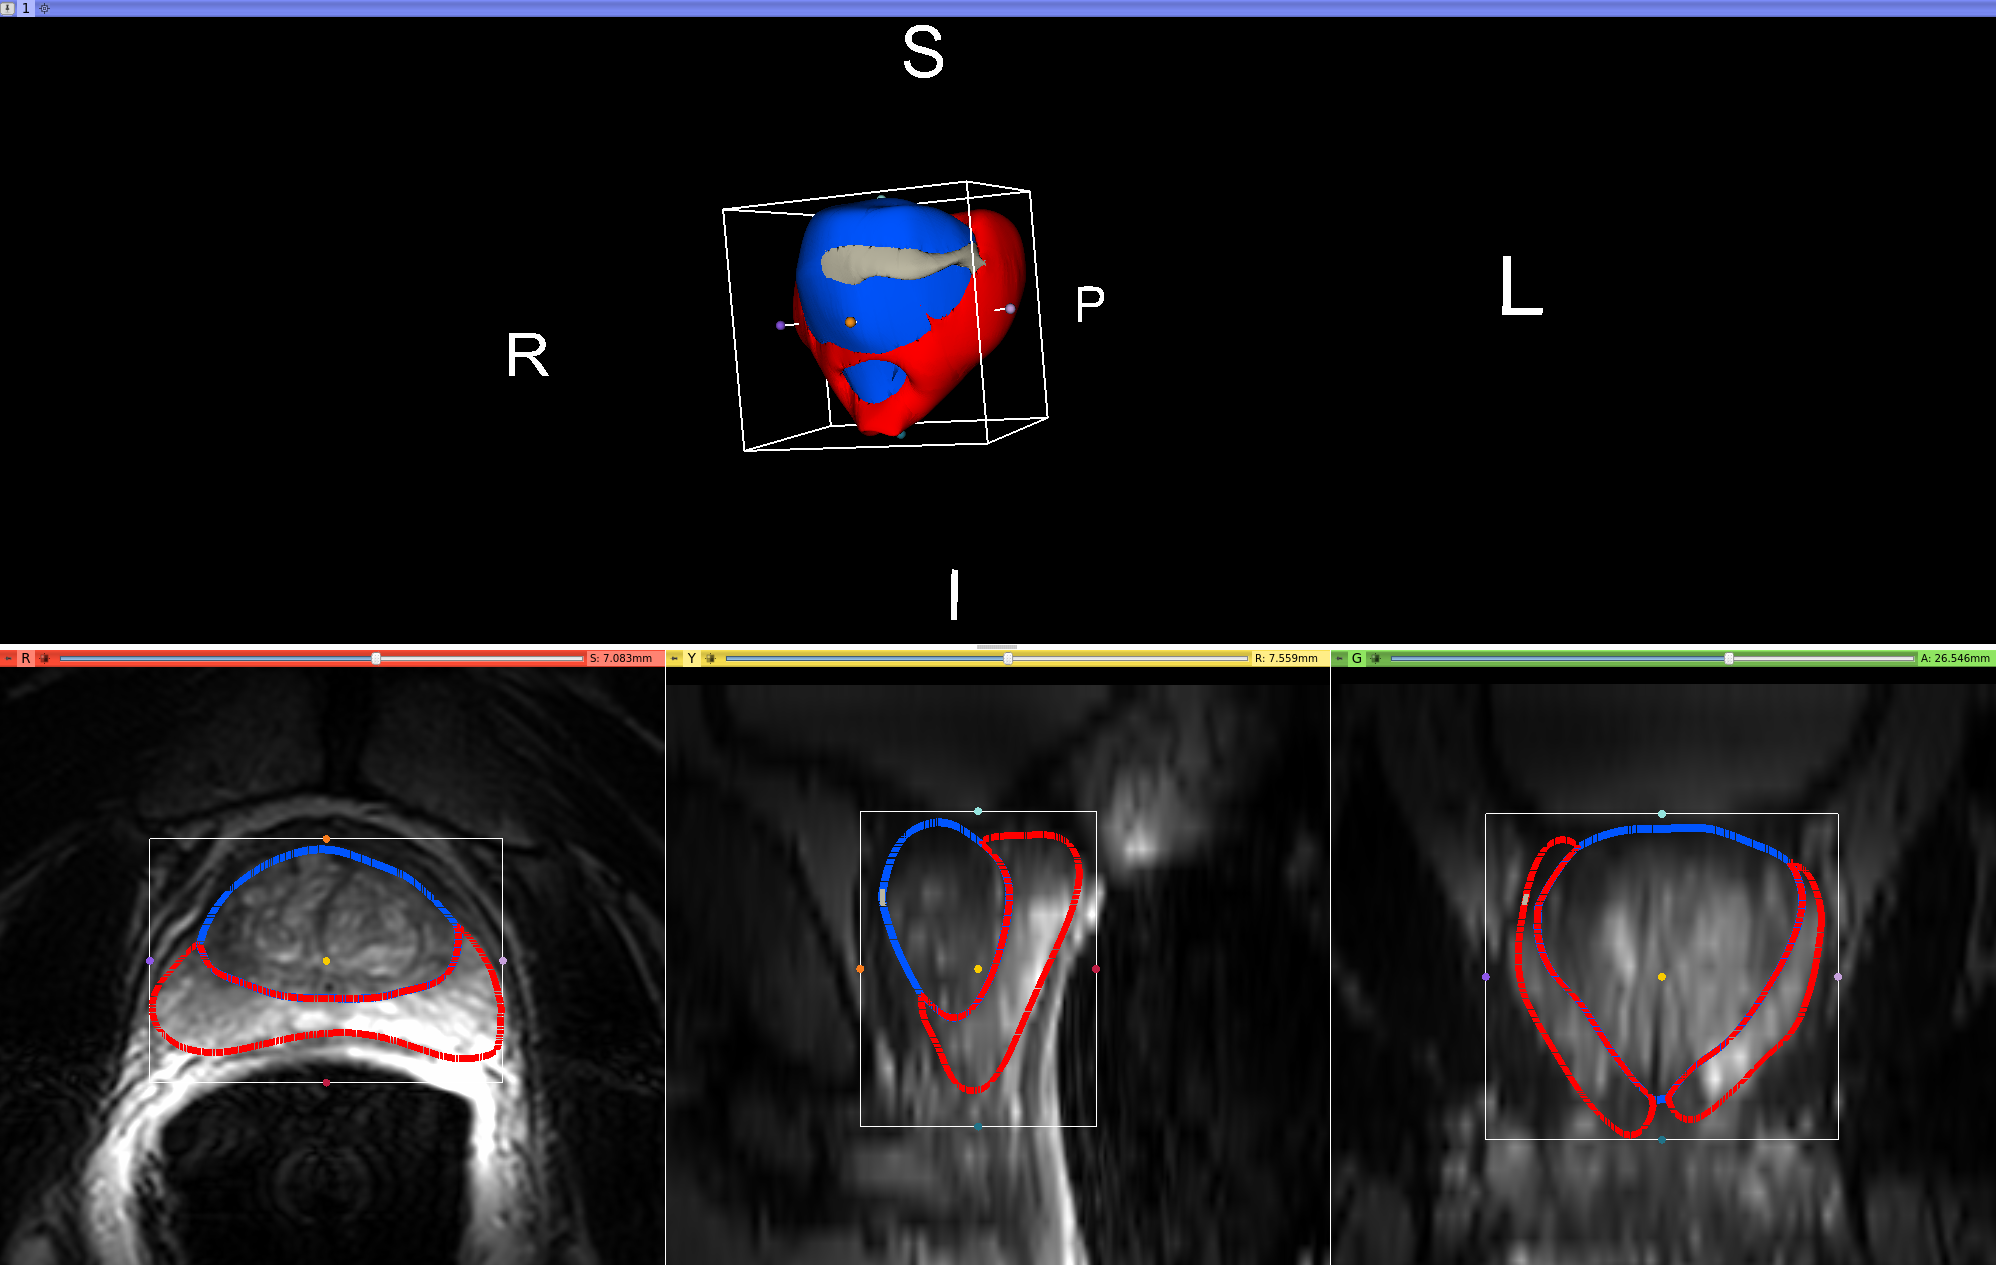
\includegraphics[width=1.0\textwidth]{tyler/MR_segs_methods.png}
\caption{Representative MR T2WI segmentations and rendered volume performed in
    3D Slicer, with the peripheral zone (PZ) being delineated in red, the
    central gland (CG) being delineated in blue, and the anterior fibromuscular
    stroma (AFS) being shown in gray.  The AFS was combined with the PZ for
    quantitative analyses shown herein.  The native imaging plane for
    segmentation is the axial view, shown in the bottom left image.  The bottom
    middle and right images show the projections of the rendered model segment
    outlines in the sagittal and coronal views, respectively. 3D view of the rendered volume shows anatomical markers for patient left (L), right (R), superior (S), inferior (I), and posterior (P).}
\label{fig:mr_segs_vol} 
\end{figure}
